\chapter{Transformation to Standard
  Normal}\label{transformation-to-standard-normal}

Values of the Standard Normal Gaussian (\(Z = \mathcal{N}(0,1)\))
percentiles are tabled everywhere (see for example Fig.~\ref{fig:normpercentile}) and from them it is possible to
derive the values relative to any other Gaussian distributions.

\begin{figure}[tb]
\centering
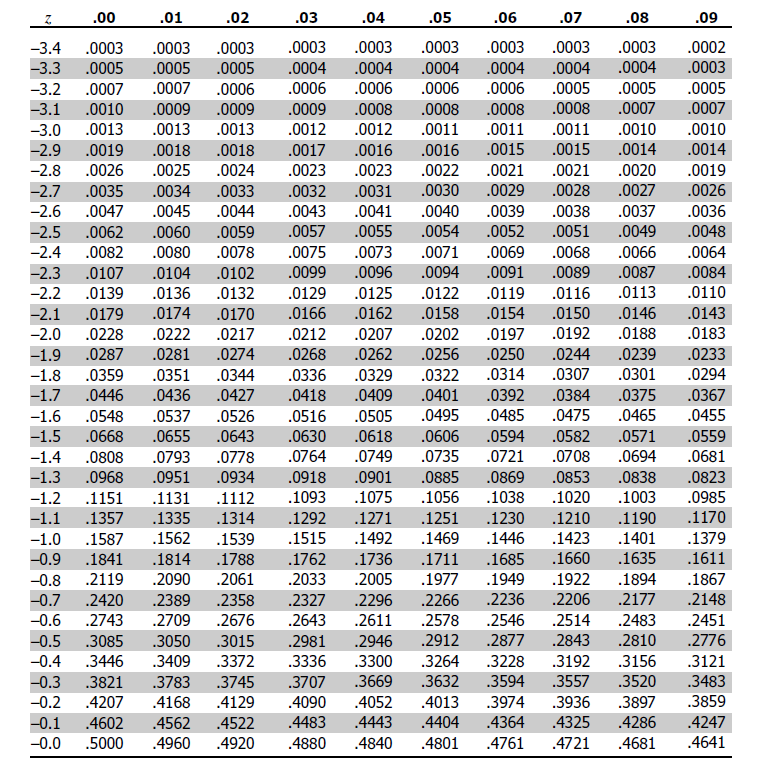
\includegraphics[width=1.\textwidth]{figures/norm_gauss_percentile}
\label{fig:normpercentile}
\end{figure}

Given a generic Gaussian \(\mathcal{N}(\mu , \sigma)\), we can go back
to the standard Gaussian as:

\begin{equation}Z= \frac{X-\mu}{\sigma}\end{equation}

and from the table above get the correct percentile.

Assume you need to know the percentage of a generic Gaussian
\(\mathcal{N}(\mu=20 ,\sigma=5)\) above \(X=30\):

\[Z=\frac{X-\mu}{\sigma} = \frac{30-20}{5}=2\]

So we just need to check on the table above the percentage related to
\(Z=2\) which is 2.28\% (look at row -2.00, column .00). Thus, 2.28\% of
the population with a normal distribution
\(\mathcal{N}(\mu=20 ,\sigma=5)\) lies above \(X=30\):

\[P(X>30)=P(Z>2)=0.0228\]

Conversely if you need to know the 1\% percentile of a generic Gaussian
\(\mathcal{N}(\mu=20 ,\sigma=5)\), first look for .01 in the table above
and check the corresponding \(Z\) value (-3.1). Finally inverting the
above formula get the right value of the percentile:

\[ X= \sigma Z + \mu = 5\cdot -3.1 + 20 = 4.5 \]
